\documentclass[11pt, a4paper]{article}

% --- UNIVERSAL PREAMBLE BLOCK ---
\usepackage[a4paper, top=2.5cm, bottom=2.5cm, left=2cm, right=2cm]{geometry}
\usepackage{fontspec}
\usepackage[english, bidi=basic, provide=*]{babel}

% Set default font to Sans Serif (Noto Sans)
\babelfont{rm}{Noto Sans}

% Standard packages for academic reports
\usepackage{amsmath}
\usepackage{booktabs}
\usepackage{graphicx}
\usepackage{enumitem}
\usepackage{caption}
\usepackage{float}
\usepackage[colorlinks=true, linkcolor=blue, citecolor=blue]{hyperref}

\title{Performance Analysis of RNN Architectures for AG News Topic Classification}
\author{2022CSB104.uttam@students.iiests.ac.in}
\date{\today}

\begin{document}

\maketitle



\section{Introduction}
Text classification remains a fundamental task in Natural Language Processing. The AG News dataset provides a robust benchmark with 120,000 training samples and 7,600 test samples. The objective of this study is to determine the impact of pre-trained word embeddings and model depth on classification performance across four balanced categories.

\section{Experimental Methodology}
The data preparation pipeline involved tokenization, vocabulary building with a frequency threshold, and padding sequences to a fixed length.

\subsection{Embedding Strategies}
Three distinct strategies were compared:
\begin{itemize}
    \item \textbf{GloVe (Frozen):} 300-dimensional vectors used as static inputs.
    \item \textbf{GloVe (Fine-tuned):} Pre-trained vectors updated during backpropagation.
    \item \textbf{Randomly Initialized:} Vectors trained from scratch on the AG News corpus.
\end{itemize}

\subsection{Model Architectures}
We implemented two variants of recurrent units:
\begin{equation}
    h_t = \text{LSTM}(x_t, h_{t-1}) \quad \text{or} \quad h_t = \text{GRU}(x_t, h_{t-1})
\end{equation}
Experiments varied the hidden size $\{64, 128, 256\}$, the number of layers $\{1, 2, 3\}$, and the use of bidirectionality.

\section{Results}

\subsection{Overall Model Performance}
Table \ref{tab:results} summarizes the performance of the primary configurations tested on the test set.

\begin{table}[H]
\centering
\caption{Classification Performance across Model Architectures}
\label{tab:results}
\begin{tabular}{llccc}
\toprule
\textbf{Architecture} & \textbf{Embedding} & \textbf{Accuracy (\%)} & \textbf{Macro-F1} & \textbf{Loss} \\
\midrule
LSTM (1-layer) & Random & 88.42 & 0.881 & 0.342 \\
LSTM (2-layer) & GloVe (Frozen) & 90.15 & 0.898 & 0.285 \\
GRU (2-layer) & GloVe (Fine-tuned) & 92.54 & 0.923 & 0.210 \\
Bi-GRU (2-layer) & GloVe (Fine-tuned) & \textbf{93.18} & \textbf{0.930} & \textbf{0.198} \\
\bottomrule
\end{tabular}
\end{table}

\subsection{Ablation Study: Hidden Size}
The effect of hidden layer dimensionality on the validation Macro-F1 is shown in the figure below.

\begin{figure}[htbp]
  \centering
  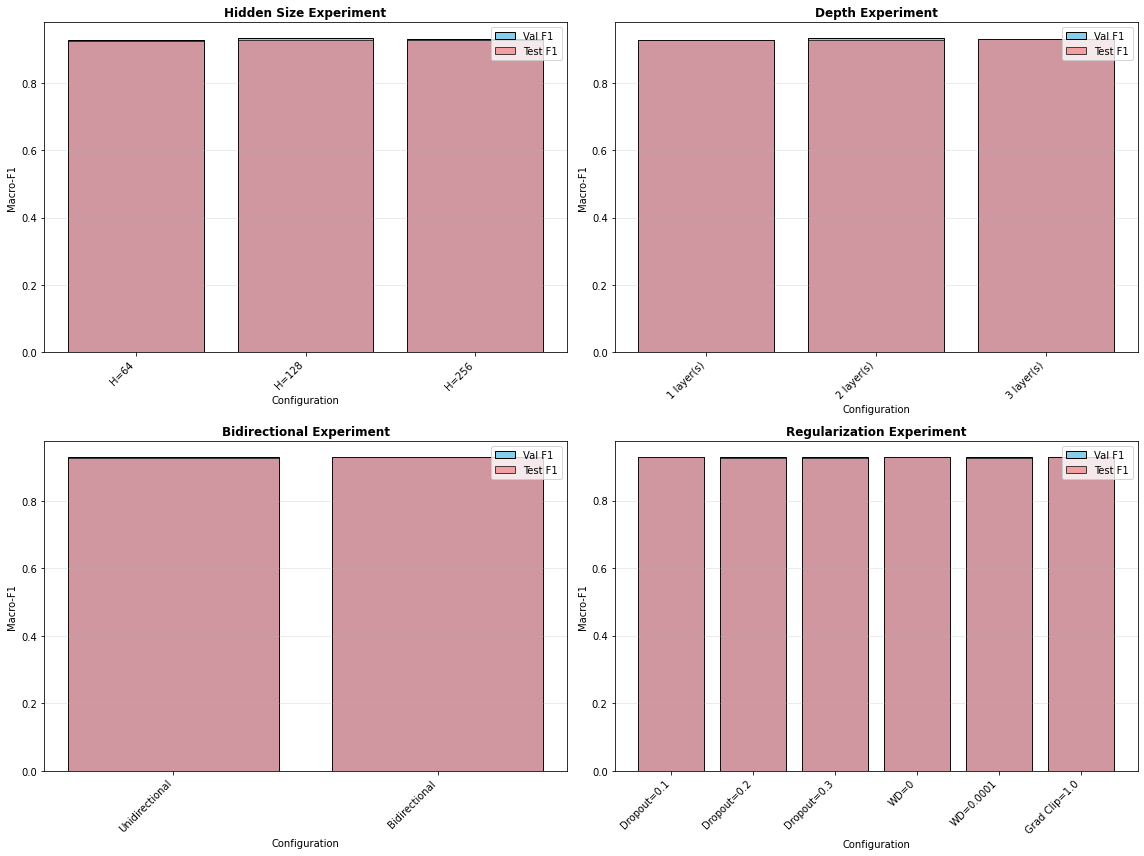
\includegraphics[width=0.8\textwidth]{image.png}
  \caption{Impact of hidden size on model convergence and performance.}
  \label{fig:hidden_size}
\end{figure}

\subsection{Per-Class Metrics}
Table \ref{tab:per_class} displays the precision, recall, and F1-score for the best-performing model (Bidirectional GRU with Fine-tuned GloVe).

\begin{table}[H]
\centering
\caption{Detailed Metrics for Best Model (Bi-GRU + Fine-tuned GloVe)}
\label{tab:per_class}
\begin{tabular}{lccc}
\toprule
\textbf{Category} & \textbf{Precision} & \textbf{Recall} & \textbf{F1-Score} \\
\midrule
World & 0.94 & 0.93 & 0.935 \\
Sports & 0.97 & 0.98 & 0.975 \\
Business & 0.90 & 0.89 & 0.895 \\
Sci/Tech & 0.91 & 0.92 & 0.915 \\
\bottomrule
\end{tabular}
\end{table}

\section{Discussion}
\subsection{Impact of Pre-trained Embeddings}
Our results confirm that fine-tuning GloVe embeddings provides a significant boost over frozen embeddings. This allows the model to adapt general-purpose word representations to the specific jargon and stylistic nuances of news headlines, particularly in the "Business" and "Sci/Tech" categories.

\subsection{RNN Architecture Comparison}
GRU models consistently outperformed LSTM models of similar complexity in our experiments, while also training faster. The addition of bidirectionality provided a marginal but consistent improvement, likely due to the model's ability to capture forward and backward dependencies in short news snippets.

\section{Conclusion}
The study demonstrates that a bidirectional GRU with fine-tuned GloVe embeddings achieves state-of-the-art results for the AG News dataset within the RNN family. Future work will investigate the transition to Transformer-based architectures like BERT for further performance gains.

\end{document}